\chapter{Black Hole Mass and Growth Saturation}
\label{chap:gravitational_saturation}

This chapter establishes the complete mechanical lifecycle of the macroscopic black hole within Tension Field Theory. It details how mass is strictly confined to the FCC/SC phase boundary, how this boundary dynamically grows through vacuum crystallization, and how it manages spin and binary mergers without relying on spacetime curvature. Finally, it derives the absolute macroscopic limits of this growth, demonstrating that as a black hole expands, its surface gravity inevitably decays, ultimately setting the mechanical stage for universal catastrophic decompression.

\section{Phase Segregation and the Holographic Mass Location}

Since the interior core of a Black Hole exists in the Simple Cubic (SC) phase, it possesses maximum structural stiffness but zero intrinsic inertia ($\mu_{\mathrm{S}} \to 0$) because it lacks the interstitial voids required for kinematic vibration. Therefore, the inertial mass ($M$) of the Black Hole is not distributed throughout its internal volume. Instead, 100\% of the effective mass is located strictly at the Phase Boundary ($R_{\mathrm{QG}}$).

Mechanically, the mass is the physical aggregate of phase-segregated topological defects. Because these defects cannot penetrate the void-less core, they are mechanically displaced by the advancing crystallization front and pinned against the boundary. Thus, a Black Hole is mechanically a solid, inertially passive, phase-locked crystal of maximum tension, enveloped by a hyper-compressed Face-Centered Cubic (FCC) boundary shell containing the entire dynamic mass of the system. \textit{(Note: This aligns exactly with \hyperref[part:one]{Part~\ref{part:one}}, where mass was established as a topological defect strictly on the boundary layer).}

\vspace{0.5em}
\noindent\textbf{The Singular Boundary Layer ($r_{\mathrm{D}}$)}
The topological mass does not stack into multiple volumetric layers under pressure; it is mathematically confined to the absolute first layer of active FCC nodes ($r_{\mathrm{D}}$) touching the core. This is guaranteed by the linear scaling law of the Event Horizon.

At the fundamental limit to form a micro black hole, the system consists of a single saturated cell with radius $R_{\mathrm{QG}} = r_{\mathrm{D}}$. Its volumetric density is the convergence limit ($\rho_{\mathrm{QG}}$):
\begin{equation}
    M \approx \rho_{\mathrm{QG}} \cdot r_{\mathrm{D}}^3
\end{equation}

Because the macroscopic Event Horizon radius scales strictly linearly with mass ($M \propto R_{\mathrm{QG}}$), the macroscopic mass is the fundamental seed mass multiplied by the radial scaling factor ($R_{\mathrm{QG}}/r_{\mathrm{D}}$):
\begin{equation}
    M \approx (\rho_{\mathrm{QG}} \cdot r_{\mathrm{D}}^3) \left( \frac{R_{\mathrm{QG}}}{r_{\mathrm{D}}} \right)
\end{equation}
\begin{equation}
    M \approx \rho_{\mathrm{QG}} \cdot r_{\mathrm{D}}^2 \cdot R_{\mathrm{QG}}
\end{equation}

This exact geometric formula dictates that as the Black Hole grows, its surface area ($A \propto R_{\mathrm{QG}}^2$) expands exponentially faster than its mass accumulation ($M \propto R_{\mathrm{QG}}^1$). Consequently, the boundary layer actually becomes less crowded as the core expands, permanently eliminating the mechanical necessity for mass to compress into multiple radial layers. The inertia of the system remains a strictly two-dimensional topological boundary phenomenon.

\section{Black Hole Growth Mechanism (Vacuum Phase Conversion)}

\textbf{The Density Gap Problem:} In \hyperref[sec:phase_transition]{Section \ref*{sec:phase_transition}}, we established that the core density must be the Substrate Density ($\rho_{\mathrm{S}} \approx 10^{96}$ kg/m$^3$). Standard accretion of inertial matter is insufficient to generate this hyper-density at cosmic scales. Therefore, a Black Hole cannot expand solely through the accretion of localized matter; it must structurally phase-convert the surrounding Active Vacuum.

\vspace{0.5em}
\noindent\textbf{The Solution: The Crystallization Front}

The Black Hole grows by propagating a phase transition into the surrounding medium. It converts the voluminous FCC Lattice into the hyper-dense SC Substrate, effectively ``mining'' the vacuum for structural density.

\begin{enumerate}
    \item \textbf{Nucleation (The Ignition):} The initial gravitational contraction of baryonic matter (a star) acts strictly as a Catalytic Event. It provides the localized pressure required to bridge the gap from atomic density to the Convergence Density ($\rho_{\mathrm{QG}}$). Once this gap is crossed, the vacuum phase transition becomes self-sustaining. The star does not create the black hole; the star breaks the vacuum, allowing the black hole to form.
    \item \textbf{Geometric Locking:} As active vacuum nodes contact the phase-locked SC core, they are destabilized by geometric proximity. The immense tension of the core overrides the vibrational freedom of the adjacent nodes, forcing them to snap into the Latent SC configuration.
    \item \textbf{Topological Percolation (The Extrusion):} Because the newly forged SC nodes possess a geometric packing factor of $1.0$, they contain zero interstitial voids. Consequently, any pre-existing physical defects (baryonic matter or energetic waves) residing within the consumed FCC vacuum cannot be absorbed into the core. These topological defects are mechanically rejected, forcing them to percolate outward. They continuously ride the advancing crystallization front, accumulating directly on the Event Horizon to maintain the hyper-compressed boundary shell.
    \item \textbf{The Chain Reaction:} Each captured node becomes part of the phase-locked wall, extending the boundary of the core and contacting new active nodes. The crystal grows outward, continuously sweeping and percolating all active mass-energy to its surface.
    \item \textbf{Energy Conservation:} 
    \begin{itemize}
        \item \textit{Input:} The Kinetic Energy of the active vacuum node (Time/Vibration).
        \item \textit{Output:} The phase-locked structural potential energy of the substrate (Compression/Tension).
        \item \textit{Result:} The node ceases to tick ($t \to 0$) and becomes a unit of stored stress. The Black Hole is a Cosmic Battery, storing the kinetic energy of the universe as phase-locked lattice tension.
    \end{itemize}
\end{enumerate}

\vspace{0.5em}
\section{The Kinematics of Vacuum Consumption}
To formalize this phase conversion, we define the growth of the Black Hole not as standard mass-accretion, but as the strict rate of topological node creation ($N$) and mechanical horizon displacement ($R_{\mathrm{QG}}$).

\subsection{The Interior Growth Law (Node Multiplication)}
The rate at which the active Face-Centered Cubic (FCC) vacuum is structurally crystallized into phase-locked Simple Cubic (SC) Substrate nodes is governed by the net kinetic power injected into the system:
\begin{equation}
    \frac{\mathrm{d}N}{\mathrm{d}t} = \frac{\eta_{\mathrm{N}} P_{\mathrm{in}} - L_{\mathrm{out}}}{E_{\mathrm{S}}}
\end{equation}

\noindent\textbf{Where:}
\begin{itemize}
    \item $P_{\mathrm{in}}$: The injected kinematic power (from consumed matter and active vacuum).
    \item $L_{\mathrm{out}}$: The mechanical leakage (e.g., gravitational radiation or stress shedding during topological mismatch).
    \item $\eta_{\mathrm{N}}$: The nucleation efficiency (the geometric probability of an active FCC node snapping into the phase-locked SC configuration upon contact with the core).
    \item $E_{\mathrm{S}}$: The absolute structural energy capacity of a single SC Substrate node ($\approx 1.956 \times 10^9$ J).
\end{itemize}

This establishes that interior growth is strictly node-driven; the core expands only when the incoming kinetic energy exceeds the threshold required to forge new substrate geometry.

\subsection{The Kinematics of Event Horizon Phase Expansion}
Because the Event Horizon is a physical phase boundary, its macroscopic expansion requires mechanical work. The internal mechanical work exerted by the outward crystallization pressure of these newly formed SC nodes must equal the gravitational work required to expand the mass-energy of the exterior surface.

As fully derived in \hyperref[app:phase_transition]{Appendix \ref*{app:phase_transition}} (\hyperref[sec:phase_transition_horizon_expansion]{Section~\ref*{sec:phase_transition_horizon_expansion}}), equating the differential expansion power of the horizon's mass-energy ($E = M c_{\mathrm{E}}^2$) to the internal mechanical work rate (Force $\times$ Velocity) yields a strict phase-locked identity for the Horizon Surface Tension ($\tau_{\mathrm{QG}}$):
\begin{equation}
    \tau_{\mathrm{QG}} = \left(\frac{c_{\mathrm{E}}^2}{4\pi G R_{\mathrm{QG}}}\right) g_{\mathrm{QG}}
\end{equation}

This derivation proves from first principles that macroscopic horizon expansion is not a kinematic stretch of empty mathematical space, but a strict mechanical displacement. It is driven purely by the crystallization pressure of the growing SC core pressing outward against the elastic FCC vacuum.

\section{Live Boundary Dynamics Beyond Spherical Growth}

The radial growth law describes the spherically averaged motion of the saturation boundary,
\begin{equation}
    \dot{R}_{\mathrm{QG}} = \frac{G}{c_{\mathrm{E}}^2}\dot{M}.
\end{equation}

For a nonspherical or dynamically loaded black hole, the boundary may be written schematically as
\begin{equation}
    R(\theta,\varphi,t) = R_{\mathrm{QG}}(t) + \delta R(\theta,\varphi,t),
\end{equation}
where $R_{\mathrm{QG}}$ is the averaged saturation radius and $\delta R$ is the local boundary deformation.

The live FCC/SC boundary contains several coupled mechanical channels: center-of-mass motion, normal phase-front growth, tangential redistribution of boundary stress, and torsional boundary motion. Axial spin is assigned to torsional loading of the FCC/SC boundary and shear strain in the surrounding Soft Floor. In the first-order surface-shell model developed in \hyperref[app:live_black_hole_boundaries]{Appendix~\ref*{app:live_black_hole_boundaries}},
\begin{equation}
    \mathcal{J}_{\mathrm{BH}} = I_{\mathrm{surf}} \frac{v_{\mathrm{tor}}}{R_{\mathrm{QG}}},
\end{equation}
and
\begin{equation}
    a_\ast = \frac{c_{\mathrm{E}}\mathcal{J}_{\mathrm{BH}}}{GM^2} = \left( \frac{I_{\mathrm{surf}}}{M R_{\mathrm{QG}}^2} \right) \frac{v_{\mathrm{tor}}}{c_{\mathrm{E}}}.
\end{equation}

Thus, in this approximation, $a_\ast \leq 1$ follows from the finite kinematic capacity of the Soft Floor and the confinement of the angular-momentum carrier to the boundary scale.

For a circular binary with component saturation radii
\begin{equation}
    R_i = \frac{GM_i}{c_{\mathrm{E}}^2},
\end{equation}
and center-to-center separation $d$, the relative orbital velocity scale becomes
\begin{equation}
    v_{\mathrm{rel}} = c_{\mathrm{E}} \sqrt{ \frac{R_1+R_2}{d} }.
\end{equation}

The contact-scale limit $v_{\mathrm{rel}}\rightarrow c_{\mathrm{E}}$ occurs only when $d\rightarrow R_1+R_2$. It is not a universal binary velocity law.

In TFT, binary merger is the formation of a common saturated phase boundary, not the geometric limit $d=0$. A schematic bridge condition is
\begin{equation}
    \alpha_{\mathrm{bridge}} = \alpha_{\mathrm{G},1} + \alpha_{\mathrm{G},2} + \alpha_{\mathrm{dyn}} \geq 1,
\end{equation}
where $\alpha_{\mathrm{dyn}}$ denotes dynamic loading from orbital compression, shear, torsion, and nonlinear boundary deformation.

After merger, the common boundary sheds excess stress and relaxes. The ringdown stage is therefore interpreted as damped relaxation of the live FCC/SC phase boundary. A minimal linearized form is
\begin{equation}
    \frac{\partial^2 \delta R}{\partial t^2} + \Gamma_{\mathrm{QG}} \frac{\partial \delta R}{\partial t} + \omega_{\mathrm{QG}}^2\delta R = 0.
\end{equation}

The detailed surface-dynamical treatment of spin, bridge formation, stress shedding, and ringdown is given in \hyperref[app:live_black_hole_boundaries]{Appendix~\ref*{app:live_black_hole_boundaries}}. The separate Kerr-limit matching problem is formulated in \hyperref[app:kerr_limit]{Appendix~\ref*{app:kerr_limit}}.

\section{Kerr Correspondence and the Observational Surface Map}

A viable alternative to the Kerr exterior must reproduce established spin-dependent astrophysical observables without importing the geometric singularity or the empty-spacetime metric. In TFT, this is achieved through a strict continuum-mechanical closure of the rotating Soft Floor, detailed in \hyperref[app:bh_rotating_kerr_clouser]{Appendix~\ref*{app:bh_rotating_kerr_clouser}}.

Torsional loading of the FCC/SC boundary generates an exterior azimuthal shear field. Weak-field angular momentum matching enforces the standard Lense--Thirring frame-dragging rate:
\begin{equation}
    \omega_{\mathrm{drag}}(r) = \frac{2G\mathcal{J}_{\mathrm{BH}}}{c_{\mathrm{E}}^2 r^3}.
\end{equation}

Furthermore, boundary relaxation requires that transient surface deformations shed excess strain energy via gravitational wave emission until the exterior multipoles depend only on mass and spin. Under the adopted no-hair quadrupole closure, the relaxed boundary matches the Kerr quadrupole limit:
\begin{equation}
    Q_{\mathrm{TFT}} = -a_\ast^2 M R_{\mathrm{QG}}^2.
\end{equation}

Because TFT replaces the GR interior and horizon ontology, the “surface” of a rotating black hole is not a single coordinate radius. It is a layered mechanical and optical map:
\begin{equation}
    R_{\mathrm{obs}}(a_\ast) = \left\{ R_{\mathrm{QG}}, \, r_{\mathrm{sat}}, \, r_{\mathrm{cap}}, \, r_{\gamma,s_{\mathrm{br}}}, \, B_{\gamma,s_{\mathrm{br}}}, \, r_{\mathrm{ISCO},s_{\mathrm{br}}} \right\}.
\end{equation}

Here, $R_{\mathrm{QG}}$ is the mass-defined saturation scale. The actual spin-deformed physical boundary is $r_{\mathrm{sat}}(\theta, a_\ast)$. The ergosphere is mechanically replaced by the torsional capacity surface, $r_{\mathrm{cap}}(\theta, a_\ast)$, where the Soft-Floor drift speed equals the local propagation capacity. Finally, the observable photon rings ($r_{\gamma}$), shadow-impact scales ($B_{\gamma}$), and massive-particle Innermost Stable Circular Orbits ($r_{\mathrm{ISCO}}$) are derived directly from the dragged, strain-refractive Soft Floor Hamiltonian. 

This establishes a fully computable TFT replacement framework for rotating black-hole exteriors, where exact Kerr-correspondence is maintained in the weak field, leaving strong-field deviations to be governed by the nonlinear mechanics of the saturated FCC/SC phase transition.

\section{The Black Hole Saturation Mass}

A Black Hole is not a static object; it is a dynamic phase boundary stable only due to the existence of a Pressure Gradient:

\begin{itemize}
    \item \textbf{Crystallization Pressure (Outward):} The mechanical force of the advancing SC phase domain converting the vacuum, driven by the geometric locking of new nodes.
    \item \textbf{Boundary Tension (Inward):} The elastic holding tension ($\tau_{\mathrm{QG}}$) of the hyper-compressed FCC boundary shell resisting the expansion, generated by the areal mass density ($\Sigma_{\mathrm{surf}}$) of the segregated defects, and supported by the ambient pressure of the surrounding vacuum.
\end{itemize}

As a Black Hole grows, it obeys a strict inverse scaling law. While its microscopic volumetric boundary density remains locally maxed at the convergence limit ($\rho_{\mathrm{QG}}$), its macroscopic Areal Mass Density ($\Sigma_{\mathrm{surf}}$) diffuses. By dividing the macroscopic mass equation derived above by the spherical surface area ($A = 4\pi R_{\mathrm{QG}}^2$), we find:
\begin{equation}
    \Sigma_{\mathrm{surf}} = \frac{\rho_{\mathrm{QG}} \cdot r_{\mathrm{D}}^2 \cdot R_{\mathrm{QG}}}{4\pi R_{\mathrm{QG}}^2} = \left( \frac{\rho_{\mathrm{QG}} \cdot r_{\mathrm{D}}^2}{4\pi} \right) \frac{1}{R_{\mathrm{QG}}}
\end{equation}

Because mass scales linearly while area scales quadratically, the segregated mass spreads thinner across the growing boundary. Consequently, the inward Boundary Tension ($\tau_{\mathrm{QG}} = \Sigma_{\mathrm{surf}} \cdot c_{\mathrm{E}}^2$) generated by this mass strictly decreases inversely with the radius ($\tau_{\mathrm{QG}} \propto R_{\mathrm{QG}}^{-1}$).

\vspace{0.5em}
\noindent\textbf{The Saturation Limit:} The growth of a Black Hole is bounded by the causal limits of the lattice. The limit is reached when the areal mass density of the Black Hole dilutes to match the ambient density of the Photon Energy-Relaxation Length ($R_{\mathrm{U}}$). At this point, the pressure gradient vanishes ($\Delta P = 0$), the Event Horizon dissolves, and the Black Hole ceases to function as a bounded object.

\vspace{0.5em}
\noindent\textbf{Derivation of the Saturation Mass ($M_{\mathrm{Sat}}$):} We derive the theoretical universal mass limit by equating the Black Hole's causal radius with the Universe's causal radius.

\begin{itemize}
    \item \textit{Black Hole Radius (Lattice Convergence Limit):} $R_{\mathrm{QG}} = \frac{GM}{c_{\mathrm{E}}^2}$
    \item \textit{Cosmic Causal Radius (Photon Energy-Relaxation Length):} $R_{\mathrm{U}} = \frac{c_{\mathrm{E}}}{\Gamma_{\mathrm{D}}}$
\end{itemize}

\noindent The Saturation Condition ($R_{\mathrm{QG}} = R_{\mathrm{U}}$):
\begin{equation}
    \frac{G M_{\mathrm{Sat}}}{c_{\mathrm{E}}^2} = \frac{c_{\mathrm{E}}}{\Gamma_{\mathrm{D}}}
\end{equation}
The Universal Closure Mass:
\begin{equation}
    M_{\mathrm{Sat}} = \frac{c_{\mathrm{E}}^3}{G \Gamma_{\mathrm{D}}}
\end{equation}

\vspace{0.5em}
\begin{minipage}{\textwidth}
\textbf{Physical Interpretation:}
\begin{itemize}
    \item \textbf{If $M < M_{\mathrm{Sat}}$:} The object is a local Black Hole (Type I) with a distinct horizon and a strong stabilizing pressure gradient.
    \item \textbf{If $M = M_{\mathrm{Sat}}$:} The object's boundary expands to encompass the entire causal volume ($\propto R_{\mathrm{U}}^3$). The localized topological defect dissolves into the contiguous global continuum, mechanically eliminating the ``Inside/Outside'' boundary.
\end{itemize}
\end{minipage}

\vspace{0.5em}
\section{Derivation of the Reservoir Radius ($R_{\mathrm{Res}}$)}
\label{sec:reservoir_radius}

To build a solid SC core the size of the Cosmic Horizon ($R_{\mathrm{U}} \approx 1.2665 \times 10^{26}$ m), the Black Hole must harvest a specific volume of vacuum nodes. Applying the strict conservation of mass ($V_{\mathrm{FCC}} \cdot \rho_{\mathrm{QG}} = V_{\mathrm{SC}} \cdot \rho_{\mathrm{S}}$), we utilize the exact phase densities derived in \hyperref[app:phase_transition]{Appendix \ref*{app:phase_transition}}:
\begin{equation}
    \frac{\rho_{\mathrm{S}}}{\rho_{\mathrm{QG}}} = \frac{5.1550 \times 10^{96} \text{ kg/m}^3}{5.2625 \times 10^{70} \text{ kg/m}^3} \approx 9.7957 \times 10^{25}
\end{equation}

The total required volume of active vacuum ($V_{\mathrm{FCC}}$) is exactly $9.7957 \times 10^{25}$ times the volume of the resulting core. Since radius scales with the cube root of volume ($R \propto V^{1/3}$), the radial multiplier is $(9.7957 \times 10^{25})^{1/3} \approx 4.6098 \times 10^8$.
\begin{equation}
    R_{\mathrm{FCC}} = R_{\mathrm{U}} \cdot (4.6098 \times 10^8) \approx (1.2665 \times 10^{26} \text{ m}) \cdot (4.6098 \times 10^8) \approx 5.8383 \times 10^{34} \text{ m}
\end{equation}

\vspace{0.5em}
\noindent\textbf{The Structural Phase Limits:} Based strictly on the mass-energy conservation of this phase transition, the active lattice must extend to a macroscopic boundary of $R_{\mathrm{Res}} \approx 5.8383 \times 10^{34}$ m to structurally support the total mass-energy of the local cosmic domain. We define this ultimate boundary as the Geometric Cosmic Horizon, which physically bounds the total Cosmic Reservoir. This mathematically confirms that the Cosmological Cycle operates perfectly between the two absolute mechanical limits of the continuum: the microscopic limit of the latent Substrate ($\ell_{\mathrm{S}} \sim 10^{-35}$ m) defines the fundamental geometric grain, while the total volumetric capacity of the active phase ($R_{\mathrm{Res}} \approx 10^{35}$ m) defines the macroscopic reservoir. 

\vspace{0.5em}
\noindent \textit{(Note: As established in \hyperref[part:one]{Part~\ref{part:one}} for the microscopic node scale, because the coefficient 5.8383 falls above the logarithmic midpoint of a base-10 scale ($\sqrt{10} \approx 3.16$), the ultimate volumetric capacity of the active vacuum is strictly classified as an order-of-magnitude scale of $R_{\mathrm{Res}} \sim 10^{35}$ m in all subsequent macroscopic expressions).}

\vspace{0.5em}
\section{The End of Gravity (Surface Acceleration)}
Standard physics assumes larger mass means stronger surface gravity. TFT reveals the opposite at the Event Horizon due to the linear scaling of the radius ($R_{\mathrm{QG}} \propto M$).

\vspace{0.5em}
\noindent\textbf{Standard Formula:} Surface Gravity at the horizon is $g_{\mathrm{QG}} = \frac{GM}{R_{\mathrm{QG}}^2}$.

\vspace{0.5em}
\noindent\textbf{TFT Substitution:} Substituting the gravitational saturation-radius relation $R_{\mathrm{QG}} = \frac{GM}{c_{\mathrm{E}}^2}$:
\begin{equation}
    g_{\mathrm{QG}} = \frac{GM}{\left(\frac{GM}{c_{\mathrm{E}}^2}\right)^2} = \frac{GM \cdot c_{\mathrm{E}}^4}{G^2 M^2} = \frac{c_{\mathrm{E}}^4}{GM}
\end{equation}

\noindent\textbf{The Result:}
\begin{equation}
    g_{\mathrm{QG}} \propto \frac{1}{M}
\end{equation}

\noindent\textbf{Implication:} As a Black Hole grows, the gravitational acceleration at its surface inversely decreases. The system is bounded by two strict mechanical limits:

\begin{itemize}
    \item \textbf{The Minimum Limit (The Micro-Black Hole):} At the fundamental node saturation limit ($M_{\mathrm{D,G}} \approx 10.033$ kg), the surface gravity reaches its absolute theoretical maximum ($g_{\mathrm{QG, \mathrm{max}}}$). The tension is perfectly concentrated on a single fundamental cell.
    \item \textbf{The Macroscopic State:} A Supermassive Black Hole has vastly weaker surface gravity because the holding tension is distributed over an immense, macroscopic surface area.
    \item \textbf{The Maximum Limit (Saturation):} When the Black Hole expands to the universal closure boundary ($R_{\mathrm{QG}} = R_{\mathrm{U}}$), the mass reaches $M_{\mathrm{Sat}}$. At this extreme, the surface gravity $g_{\mathrm{QG}}$ approaches zero.
\end{itemize}

\noindent\textbf{The Consequence:} At the cosmic scale, the Black Hole possesses no holding gradient left to maintain its boundary. The hyper-compressed boundary shell of extruded topological mass becomes too diffuse to contain the outward crystallization pressure of the phase-locked Substrate Core.

\begin{figure}[H]
    \centering
    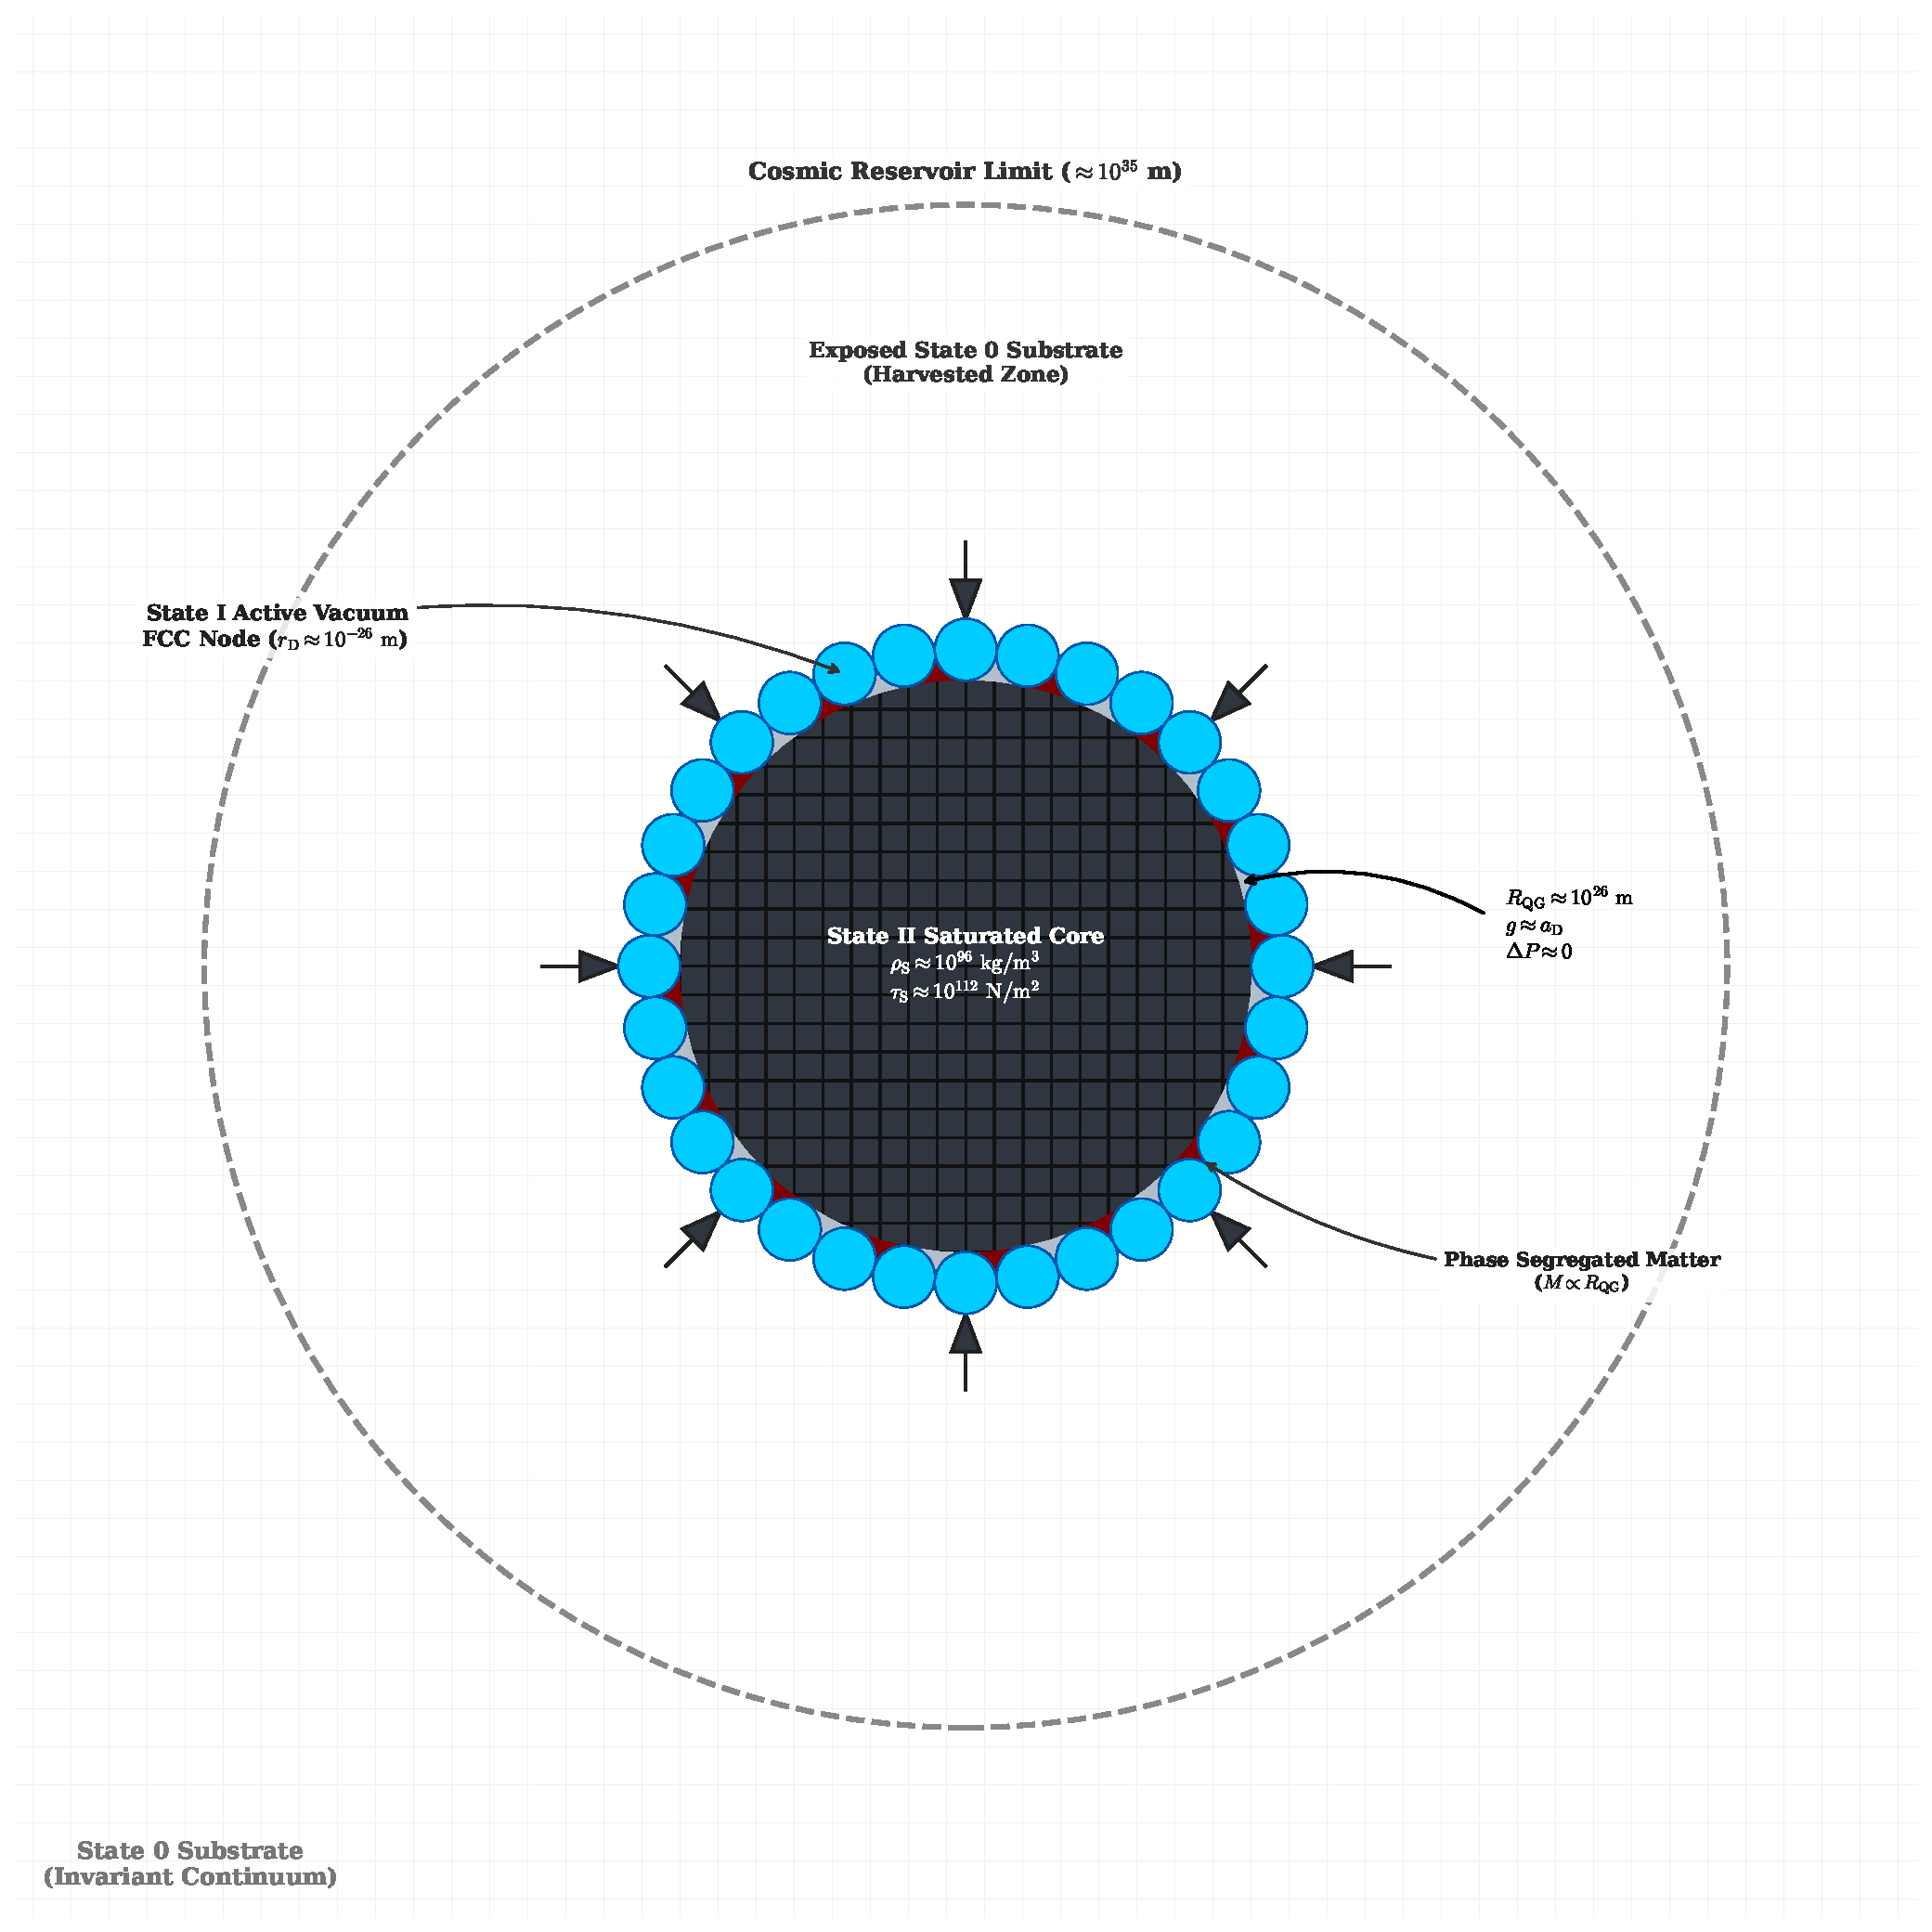
\includegraphics[width=0.9\textwidth]{Fig12_PartII_BHGrowth.pdf}
    \caption{\textbf{The Structural Mechanics of Black Hole Saturation.} The Event Horizon is a dynamic solid-state phase boundary. Following the Topological Extrusion Rule, the zero-void Simple Cubic core (State II) possesses no internal inertial mass. As the active vacuum crystallizes into this hyper-dense core, all topological defects (matter) are mechanically extruded outward and strictly confined to the interstitial voids (red) of the innermost Face-Centered Cubic (FCC) contact layer ($r_{\mathrm{D}}$). The Black Hole grows by continuously converting the voluminous active vacuum into rigid core geometry. If the object were to reach the causal mass limit ($M_{\mathrm{Sat}}$ at $R_{\mathrm{U}}$), the surface holding tension ($g$) would drop to the ambient cosmic impedance ($a_{\mathrm{D}}$), causing the containment pressure ($\Delta P$) to vanish and triggering catastrophic decompression.}
\label{fig:blackhole_growth}
\end{figure}

\section{Mechanism of Failure}

If a single Black Hole could hypothetically reach the universal closure boundary ($M_{\mathrm{Sat}}$), it would suffer an inevitable local rupture. At this scale, the restorative holding force at the surface ($g$) drops to the fundamental Cosmic Impedance Acceleration ($a_{\mathrm{D}} \approx 10^{-10}$ m/s$^2$). Because the internal gravitational binding energy is fully counteracted by the vacuum's inertial energy, the pressure gradient vanishes ($\Delta P \to 0$). The boundary would dissolve, and the super-compressed Simple Cubic (SC) core would violently decompress back into the active Face-Centered Cubic (FCC) state. 

However, it is mechanically impossible for a single Black Hole to actually reach this macroscopic saturation limit. A Black Hole does not exist in isolation; it is part of a distributed, universe-wide network of growing State II defect cores. 

Because multiple Black Holes are simultaneously consuming the active vacuum, the global geometric capacity of the FCC lattice will structurally fail long before any single core can expand to $R_{\mathrm{U}}$. Therefore, the ultimate fate of the Black Hole is not determined by its own local growth limit ($M_{\mathrm{Sat}}$), but is prematurely triggered by the global percolation fault line---resulting in the catastrophic decompression detailed in \hyperref[part:three]{Part~\ref{part:three}}.
